\chapter{Information Gathering \& Analysis}
\begin{spacing}{1}
\setlength{\parskip}{0.3in}
\graphicspath{{./Chapter3/}}

\section{Information Gathering}
Information Gathering is a very key part of the feasibility analysis process. Information gathering is both an art and a science. It is a science because it requires a proper methodology and tools in order to be effective. It is an art too, because it requires a sort of mental dexterity to achieve the best results.

\subsection{Information Gathering Tools}
For gathering information we have to go through many processes.Mainly we collect our data from:
\begin{enumerate}
\item Online Survey
\item Akash DTH FAQ section 
\end{enumerate}
And finally we are lucky to manage a meeting with a manager of akash DTH,we asked him many questions and found our required data.

\subsection{Questionnaires Analysis}
Following questions were asked in online survey to the customers 

{\bf 1.} Why do you prefer Akash DTH over cable?\newline
{\bf Tables \& Graph}
\begin{figure}[H]
	\centering
	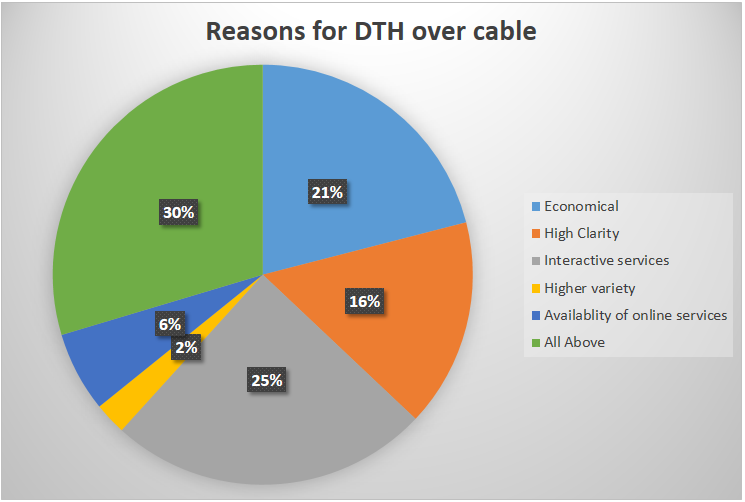
\includegraphics[width=0.5\textwidth]{fig1}
	\caption{Pie Chart of selecting reasons for DTH over cable}
	\label{fig:PieChart1}
\end{figure}
{\bf Conclusion:}\newline
Most of the Customer prefer Akash DTH over cable because of economical friendly and High quality performance which is far better than cable.

{\bf 2.} How much do you pay for your Akash DTH connection per month?\newline
{\bf Tables \& Graph}\newline
\begin{figure}[H]
	\centering
	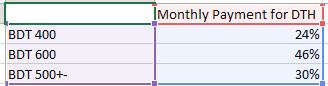
\includegraphics[width=0.8\textwidth]{fig2_1}
	\caption{Table for user's monthly payments percentage}
	\label{fig:Table1}
\end{figure}
\begin{figure}[H]
	\centering
	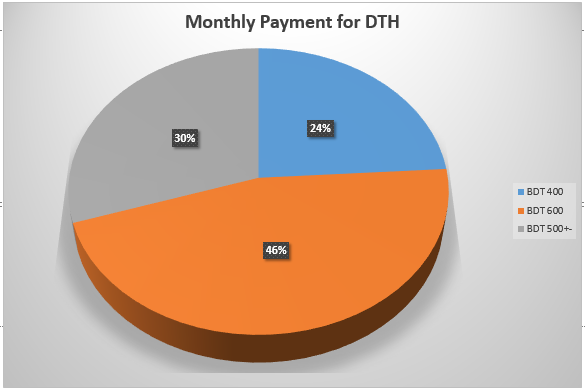
\includegraphics[width=0.8\textwidth]{fig2_2}
	\caption{Pie Chart of user's monthly payment}
	\label{fig:pieChar2}
\end{figure}
{\bf Conclusion: }\newline
Most the customer of Akash DTH purchases 400 BTD/month package

{\bf 3.} How would you rate your satisfaction from your DTH provider?\newline
{\bf Tables \& Graph}\newline
\begin{figure}[H]
	\centering
	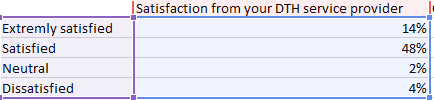
\includegraphics[width=0.8\textwidth]{fig3_2}
	\caption{Table for user's ratings}
	\label{fig:Table2}
\end{figure}
\begin{figure}[H]
	\centering
	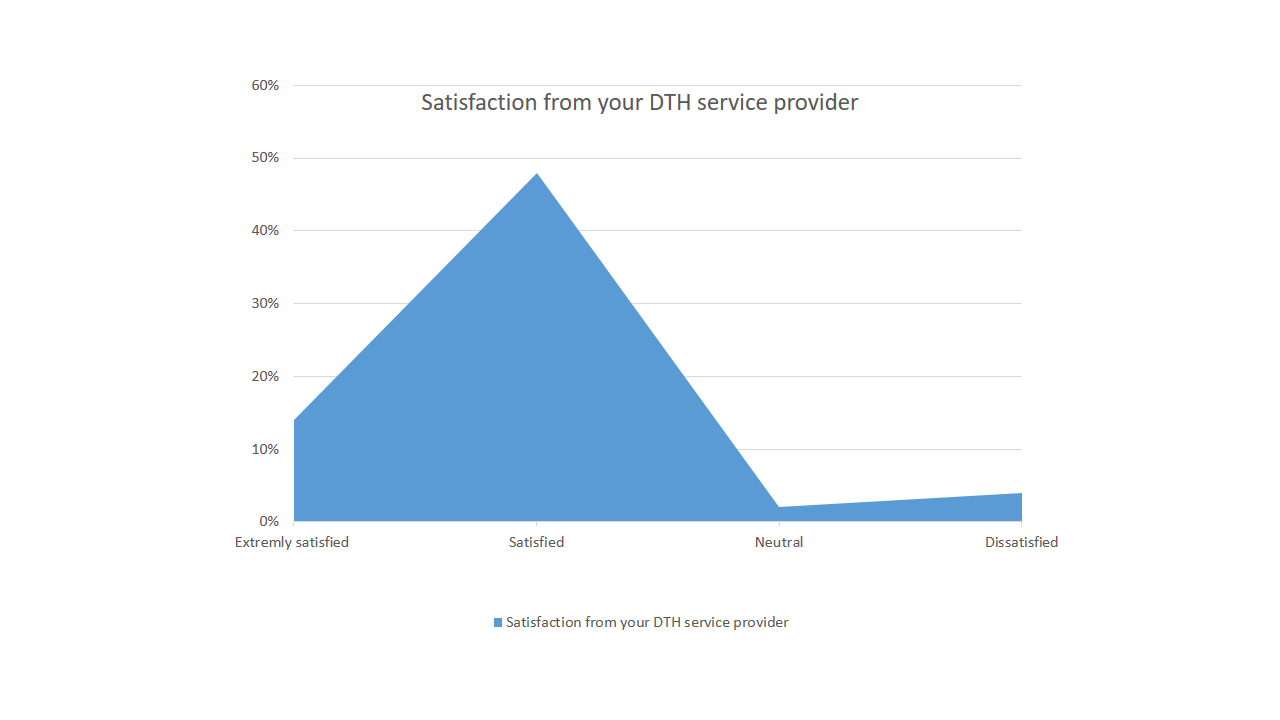
\includegraphics[width=0.8\textwidth]{fig3_1}
	\caption{Graph of user ratings}
	\label{fig:g1}
\end{figure}
{\bf Conclusion: }\newline
Maximum number of customers are satisfied with akash DTH provider.

{\bf 4.} How many channels do you get in your akash DTH package?\newline
{\bf Tables \& Graph}\newline
\begin{figure}[H]
	\centering
	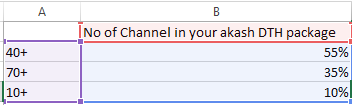
\includegraphics[width=0.8\textwidth]{fig4_1}
	\caption{Table for number of channels in packages}
	\label{fig:Table3}
\end{figure}
\begin{figure}[H]
	\centering
	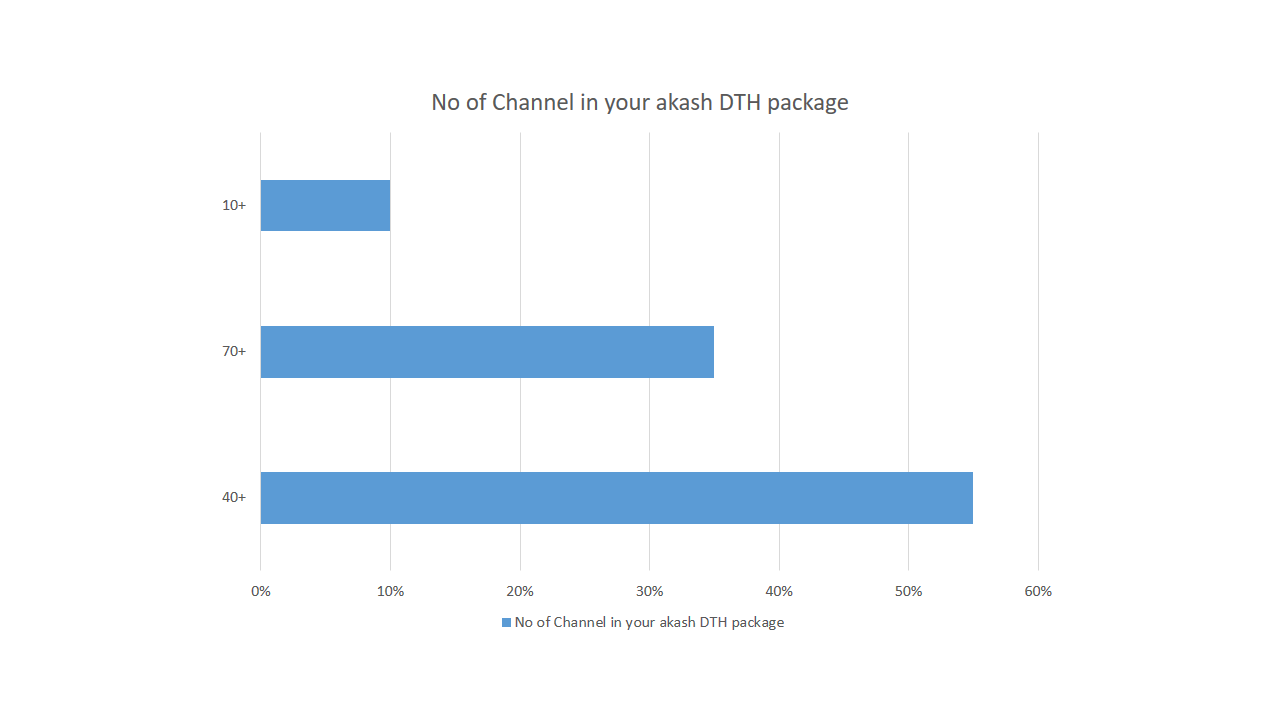
\includegraphics[width=\textwidth]{fig4_2}
	\caption{Barchart showing number of channels in user's packages}
	\label{fig:bar1}
\end{figure}
{\bf Conclusion: }\newline
Akash Basic Package serves 40+ channel which is standard for most of the customers.

{\bf 5.} Do you easily get recharge your akash DTH?\newline
{\bf Tables \& Graph}\newline
\begin{figure}[H]
	\centering
	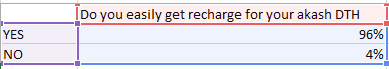
\includegraphics[width=0.8\textwidth]{fig5_1}
	\caption{Table for users percentage with ease of recharge}
	\label{fig:Table4}
\end{figure}
\begin{figure}[H]
	\centering
	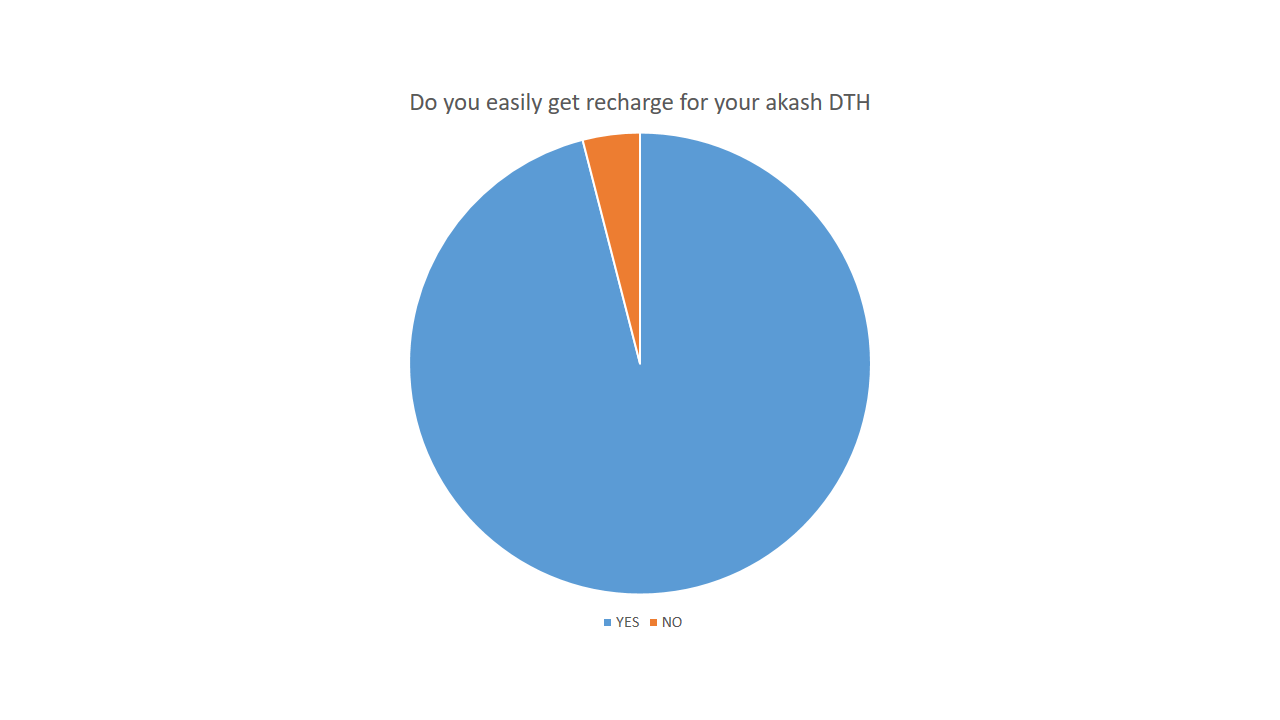
\includegraphics[width=0.8\textwidth]{fig5_2}
	\caption{Pie chart showing users with ease of recharge}
	\label{fig:pie3}
\end{figure}
{\bf Conclusion: }\newline
Akash DTH provide every types of payment accaess in Bangladesh.example : Bkash,Rocket,DBBL,Nagad,Bank Payment,Card Payment etc.So it is too much easy for most of the customer.

\section{Overview of Existing System}
\begin{figure}[H]
	\centering
	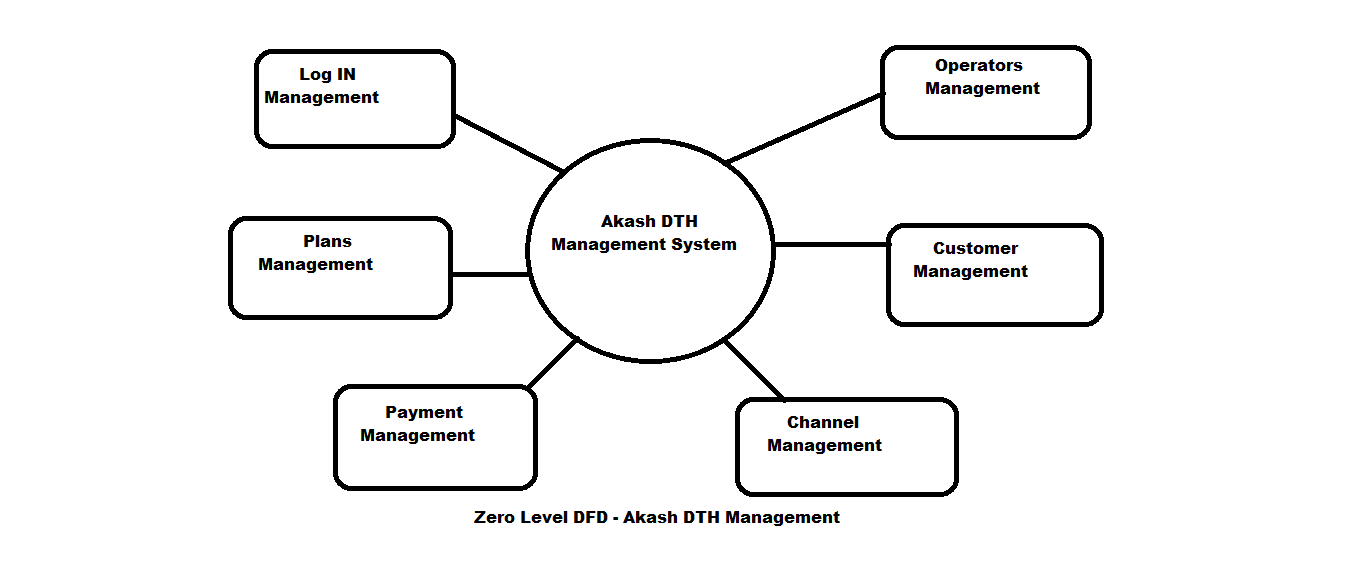
\includegraphics[width=1.2\textwidth]{DFD1}
	\caption{Akash DTH Management - Zero Level DFD}
	\label{fig:dfd1}
\end{figure}
\begin{figure}[H]
	\centering
	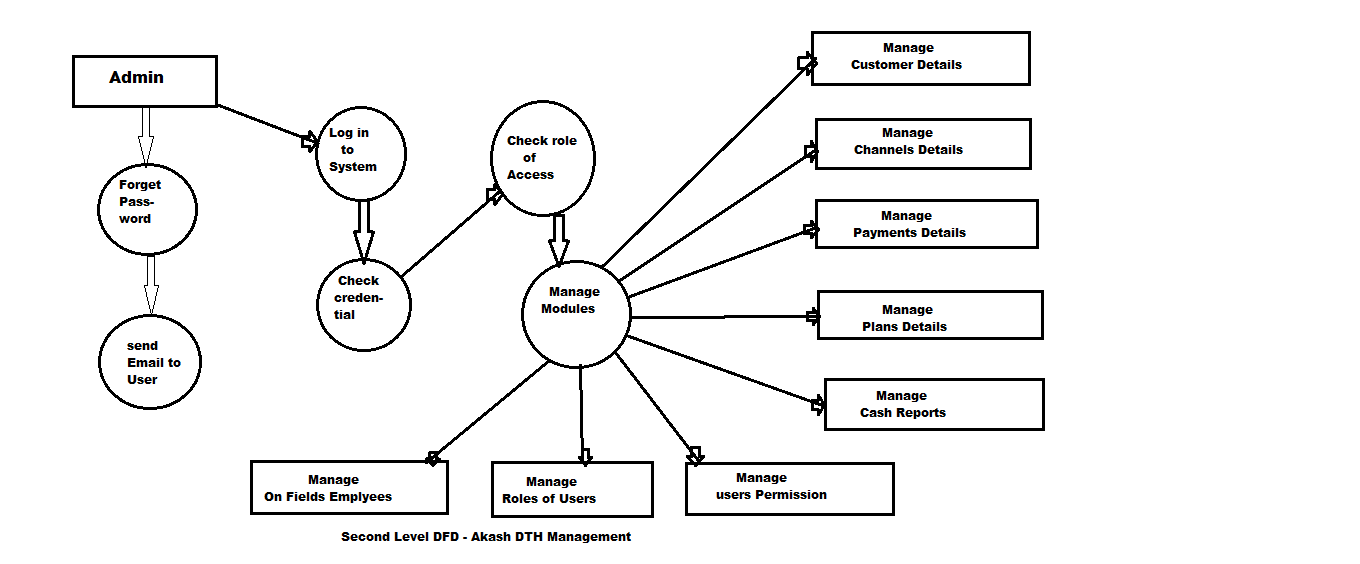
\includegraphics[width=1.2\textwidth]{DFD2}
	\caption{Akash DTH Management - Second Level DFD}
	\label{fig:dfd2}
\end{figure}
\subsection{Description of DFDs}
DFD is a most important Diagram for any System Management.Akash DTH maintains a well structured DFD Diagram for their management.Initially Akash DTH divided their management into several sub management module.The Head management managers control the sub management modules.In each sub-management module there is a group of people to manage field level employees.

\subsection{Customer Management Module}
customer management module is responsible for any types of customers complains,they generally collect data from customer phone call or physical investigation,generally they propose the upcoming customers requirements and plans.All other sub-modules works in the same flow. 

\subsection{Channel Management Module}
Channel Management Module is a vital management module.They have to conscious about customer requirements,which types of channels are mostly liked by customer. They have to Organize channels package which will satisfy customer requirements.

\subsection{Log In Management Module}
Log in management module is a small part of Akash DTH management module.A small group of tech-employee manage the Authorization of access in Akash DTH server.

\subsection{Payment Management Module}
Payment management module is the second most vital management module.They have to ensure that every customer pays their monthly bill,if any customer didn't pay his bill then they are responsible for convince the customer to pay the bill as early as possible or the will disconnect their service, and they also collaborate with different various bill payment companies to manage akash bill payment most easily.

\subsection{Plans Management Module}
Plans Management Teams discover various types of package to attract customers. 

\section{Conclusion}
We primarily collect those data from customers of akash DTH in google survey forms and in FAQ section of akash DTH webpage.And plot those data to generate diagrams,we generate DFD diagram discussing with top level managers of Akash DTH company.They share their overview system flow in a Zoom meeting and we are able to built such DFD. 

\end{spacing}
